\chapter{Présentation du projet}

\section{Idée de départ}

L'idée directrice de notre TPE est la suivante : la capture de donnée météorologique et le transfère de ces données sur un site Web accessible à tous. Nous voulions créer un système qui permet à l'utilisateur de connaître la température ainsi que la pression d'un environnement à distance. Ce type de produit existe déjà sur le marché de la domotique mais ils stockent les données sur une carte SD (comme ceux de la marque Testo, qui coûte plus d'une centaine d'euros).

\begin{figure}[!h]
	\centering
	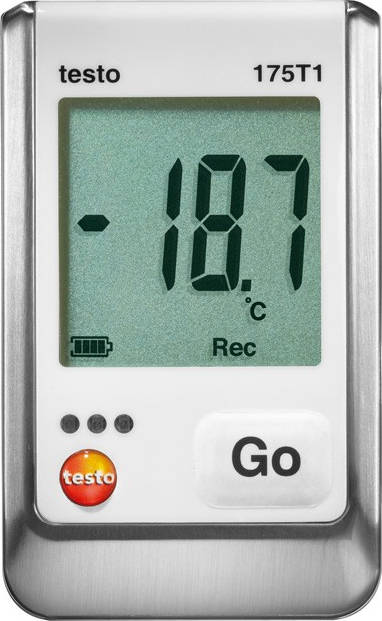
\includegraphics[height=.3\linewidth]{Images/Testo}
	\hspace{2cm}
	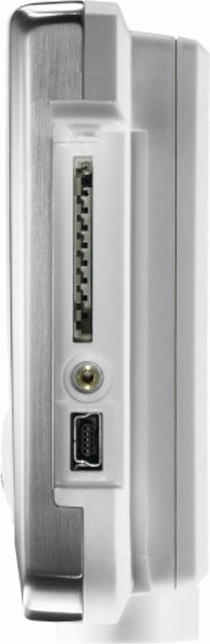
\includegraphics[height=.3\linewidth]{Images/Testo_profil}
	\caption[Le testo 175 T1]{Le testo 175 T1 (prix : \SI{150}{\EUR} TTC)}
\end{figure}

Nous avons voulu innover en stockant les relevés sur une base de données en ligne. De plus, notre projet relève non seulement la température mais aussi la pression. Nous avons aussi essayer de réduire les coûts.

Nous avons donc penser à utiliser un microcontrôleur relier à un capteur qui enverra les données vers une base de donnée. Ensuite, un site Web ira chercher les données sur cette base. Nous présenterons rapidement les éléments citées dans la synoptique et approfondirons les sujets dans les différentes parties du dossier.

\section{Analyse fonctionnelle}

Nous nous sommes donc penchés sur les caractéristique de nous devions mettre en œuvre pour arriver à mener à bien notre projet.

\subsection{Méthode APTE}

Dans un premier lieu, nous nous sommes demandés pourquoi, comment et pour qui cela pourrait servir. Nous avons donc utilisé la méthode dite \og méthode APTE \fg{} qui à pour but de déterminer l'utilité de notre projet. Au début, nous avons créés le diagramme bête à corne suivant.

\begin{figure}[!h]
	\centering
	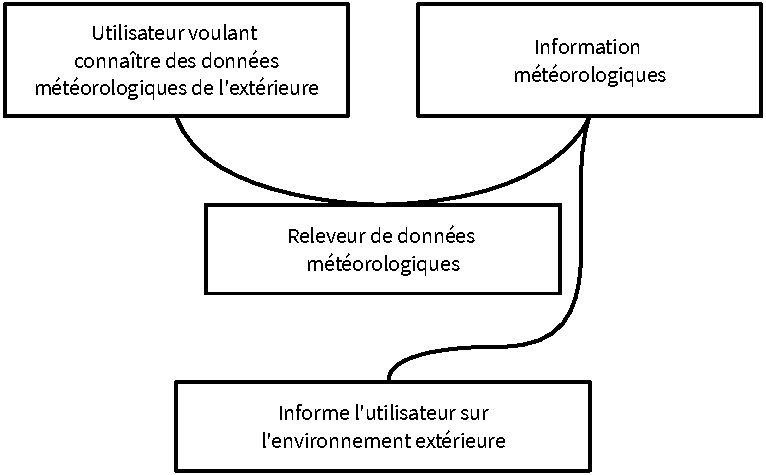
\includegraphics[width=.6\linewidth]{Images/Diagramme_APTE}
	\caption{Diagramme bête à corne de notre projet}
\end{figure}

Nous pouvons donc penser que les données météorologiques que nous recueillerons servirons à l'utilisateur. Celui-ci pourra alors être informé de la température et de la pression atmosphérique d'une pièce ou d'un extérieur en fonction de l'utilisation faite par celui qui s'en servira.

Ensuite, il a fallu nous poser quelques questions sur ce qui pourrait conduire la disparition de ce projet. Il pourrait, par exemple, naître un nouveau projet qui puissent capter des données plus précises ou plus fidèles, qui puisse stocker plus de données, \dots{} Mais pour l'instant, nous n'avons pas vu d'autre produit comme le notre !

\subsection{Diagramme des interacteurs}

Suite à cela, nous devons déterminer toutes les fonctions que réalisera notre projet et ses interactions avec l'extérieur. Ainsi, nous avons réalisé le diagramme des interacteurs ou diagramme \og pieuvre \fg{} suivant.

\begin{figure}[!h]
	\centering
	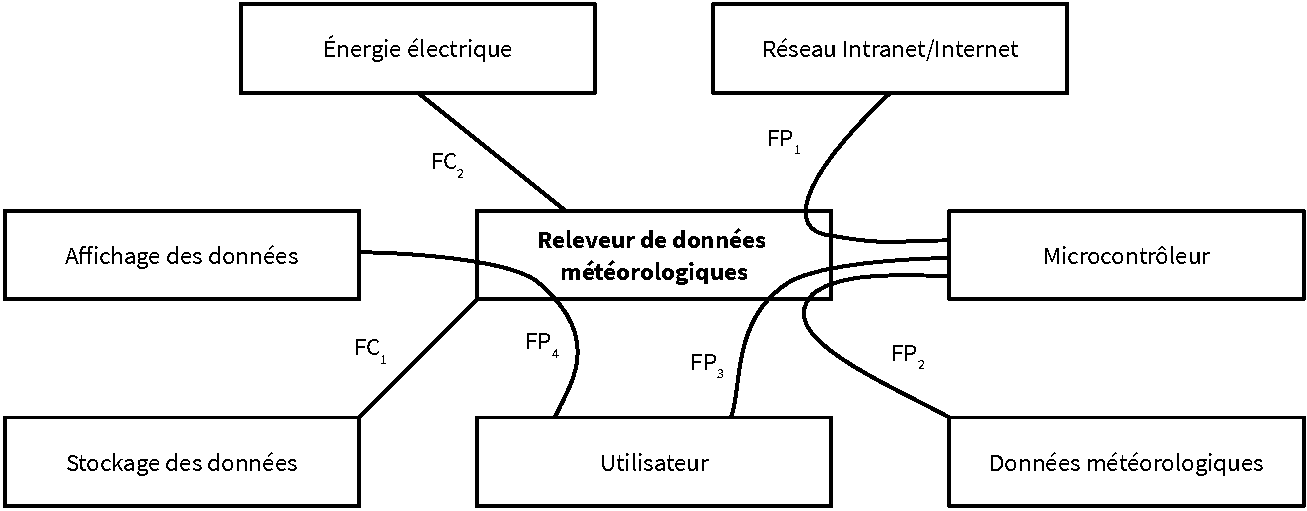
\includegraphics[width=\linewidth]{Images/Diagramme_pieuvre}
	\caption{Diagramme des interacteurs}
\end{figure}

Ainsi, sept interacteurs ont été trouvé et il en découle quatre fonctions principales et deux fonctions contraintes.

\subsection{Cahier des charges fonctionnel}

Enfin, pour terminer notre analyse fonctionnelle, nous avons regroupé toute nos caractéristiques et nos fonctions pour former un cahier de charges fonctionnel (voir tableau \ref{table:cdcf}).

\begin{sidewaystable}
	\renewcommand{\tabularxcolumn}[1]{m{#1}}
	\begin{tabularx}{\linewidth}{cXXlc}
		\toprule
		\multicolumn{2}{c}{\bfseries Fonctions} & \multicolumn{1}{c}{\bfseries Critères} & \multicolumn{1}{c}{\bfseries Niveaux} & \bfseries Fléxibilité \\
		\midrule
		$\mathrm{FP}_1$
			& Doit pouvoir communiquer des informations sur le réseau Intranet/Internet
			& Prise RJ45 et accès au réseau de lycée ou réseau local & aucun & aucun \\
		\midrule
		\multirow{2}*{$\mathrm{FP}_2$}
			& \multirow{2}\hsize{Doit pouvoir capter des données météorologiques}
			& Capteur de température & Précision à \SI{1}{\celsius} & \multirow{2}*{$\mathrm F_2$} \\
			& & Capteurs de pression & Précision à \SI{10}{\hecto\pascal} \\
		\midrule
		\multirow{3}*{$\mathrm{FP}_3$}
			& \multirow{3}\hsize{Doit être facile d'installation et d'utilisation, être sécurisé pour l'utilisateur}
			& Boîtier de protection & Étanche & $\mathrm F_0$ \\
			& & Indicateur de mise en marche & Voyant (LED) & $\mathrm F_1$ \\
			& & Raccord au réseau facile & Câble et prise RJ45 (connexion filaire) & $\mathrm F_0$ \\
		\midrule
		$\mathrm{FP}_4$
			& Données doivent être visible par l'utilisateur
			& Site Web avec langage de programmation & Espace inférieur à \SI{10}{\mega\octet} & $\mathrm F_2$ \\
		\midrule
		$\mathrm{FC}_1$
			& Doit pouvoir transférer les données sur un moyen de stockage
			& Base de données & Espace inférieur à \SI{10}{\mega\octet} & $\mathrm F_2$ \\
		\midrule
		$\mathrm{FC}_2$
			& Doit utiliser l'électricité pour s'alimenter en énergie & Électricité courante suivie d'un transformateur à courant continue & Tension de \SIrange{5}{12}{\volt} & $\mathrm F_0$ \\
		\bottomrule
	\end{tabularx}
	\caption{Le cahier des charges fonctionnel}
	\label{table:cdcf}
\end{sidewaystable}

Nous avons donc déterminé, en fonction de nos attentes, les critères pour pouvoir réaliser le projet. Le niveau correspond à la valeur du critère, par exemple, le capteur de température doit être au moins précis à \SI{1}{\celsius}. Ensuite, plus la flexibilité d'un niveau est faible, moins on peut le modifier. Nous pouvons donc voir, par exemple, que pour la température, on autorise une flexibilité de 2 ce qui veut dire que l'on autorise un précision un peu plus petite. Autre exemple, pour l'esthétique, la fléxibilité est au maximum car cela n'empêchera pas les performances ou les fonctionnalités de l'objet.

\subsection{Synoptique et chaîne d'information}

Nous avons commencé à rentrer dans les détails de notre TPE en choisissant notre capteur, qui sera un capteur de température et de pression BMP180 et notre microcontrôleur sera un Arduino Uno pour pouvoir contrôler le capteur. En plus de ce microcontrôleur, nous mettrons un Arduino Ethernet V2.0 qui nous permettra d'envoyer les données sur la base de donnée qui se situera sur un serveur qui hébergera aussi le site Web. Un \emph{switch} sera installé entre l'Arduino et l'ordinateur, nous pourrons également brancher un deuxième ordinateur en tant que client (l'utilisateur final). Pour notre base de données, nous allons utiliser MySQL et, pour notre serveur Web, nous allons utiliser Apache. Le language pour le site Web sera PHP. Tous ces logiciels sont présentées dans la section \ref{section:logiciels}.

Nous avons donc représenté les interactions entre les différents composants sur un synoptique (voir figure \ref{figure:synoptique}).

\begin{figure}[!h]
	\centering
	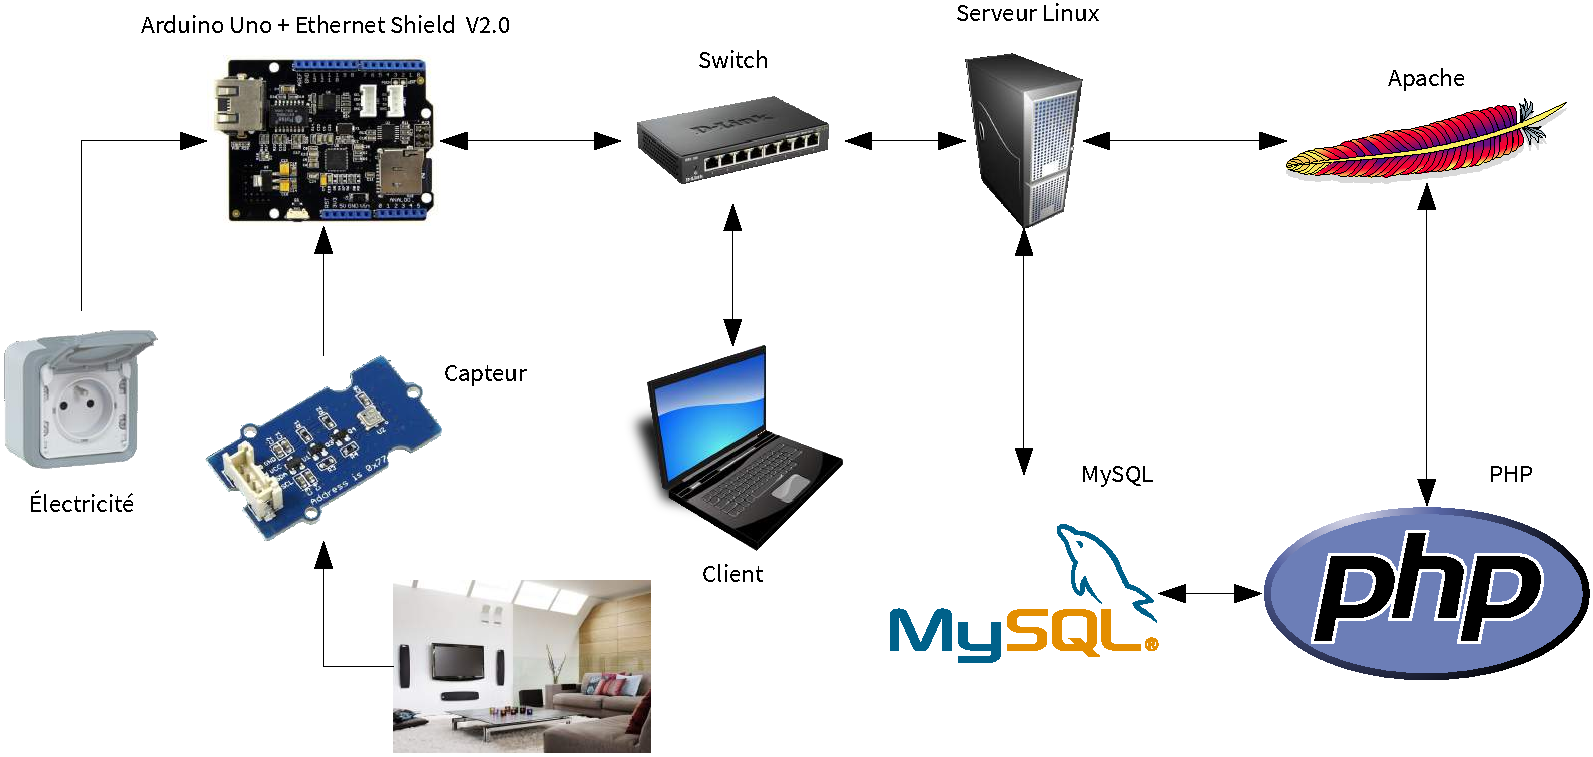
\includegraphics[width=.9\linewidth]{Images/Synoptique}
	\caption{Synoptique récapitulant tous les composants}
	\label{figure:synoptique}
\end{figure}

Enfin, nous avons déterminé notre chaîne d'information (voir figure \ref{figure:ci}), de l'acquisition de la température à l'insertion dans la base de données. La partie site Web ne figure pas car elle est indépendante de cette partie bien qu'il communique avec la base.

\begin{figure}[!h]
	\centering
	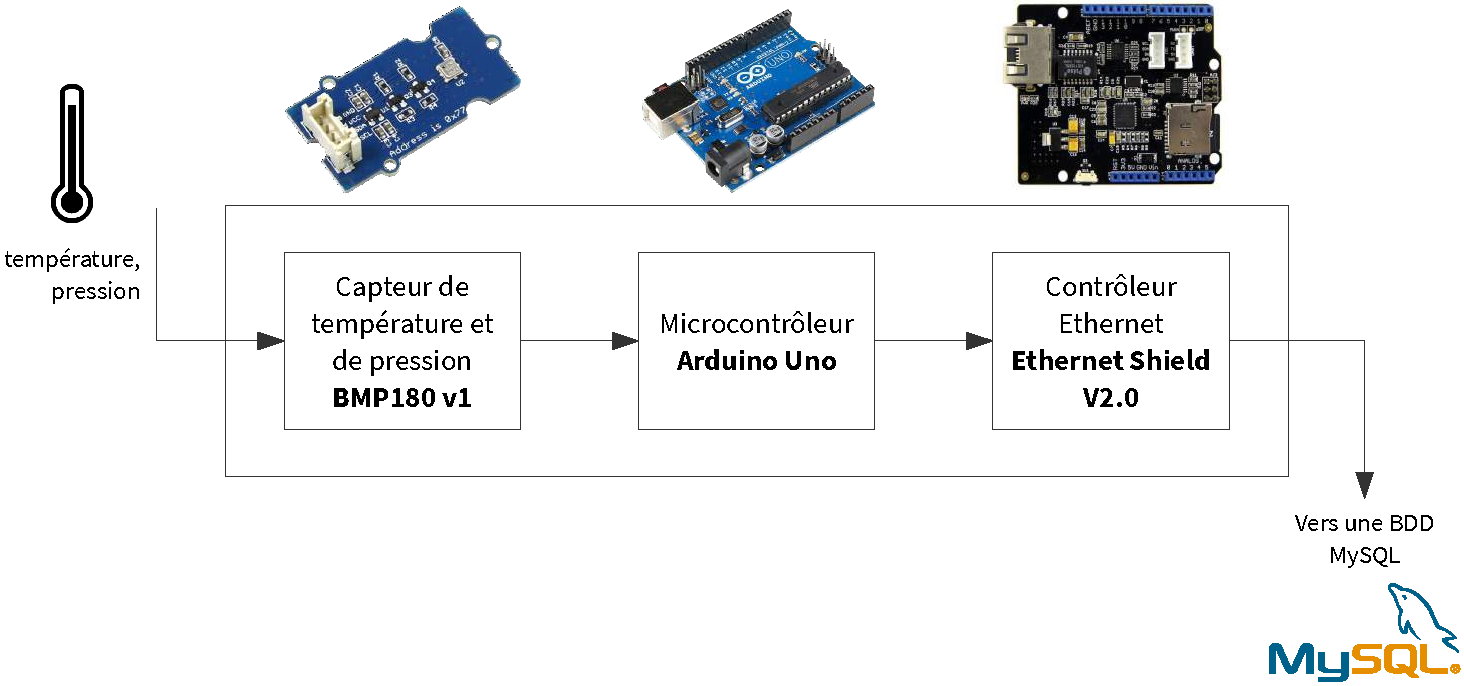
\includegraphics[width=.9\linewidth]{Images/Chaine_information}
	\caption{Chaîne d'information de la partie électronique}
	\label{figure:ci}
\end{figure}
